\documentclass[aps,pra,twocolumn,reprint,floatfix,amsmath,amssymb]{revtex4-2}
\usepackage{graphicx}
\usepackage{booktabs}
\usepackage{siunitx}
\usepackage{mathtools}
\usepackage[colorlinks=true,linkcolor=blue,citecolor=blue,urlcolor=blue]{hyperref}
\emergencystretch=2em
\begin{document}
\sloppy
\title{The Definitive Ideal SQR Gate Study}
\author{Codex}
\affiliation{Autonomous cQED Study Workspace}
\date{\today}
\begin{abstract}
This definitive study unifies the repository's selective-qubit-rotation line into one self-contained answer. It re-presents the three historical SQR baselines, normalizes their saved outputs into a single comparison frame, imports the later patched native-rich extension as the strongest new-results layer, and adds fresh cross-study diagnostics: per-manifold ideal-SQR error generators, a standalone finite-refocusing-pulse audit, explicit spectral-crowding estimates, addressed-manifold scaling fits, and a ranked practical table. The central conclusion is conditional rather than universal. Parameterized direct multitone waveforms do realize strict ideal selective qubit rotations above 0.99 on physically credible addressed windows, with the best loaded strict joint fidelity reaching 0.99899. That success does not generalize across the broader grid: the mean best strict fidelity on the structured native-rich case set is only 0.8392, far below the user's 0.95 grid-average landmark, and the harder three-manifold model with higher-order dispersive curvature still saturates around 0.9846. Echoed constructions remain compelling mainly for the relaxed conditional-phase SQR target, whose best loaded joint fidelity reaches 0.999999998. The decisive obstruction is therefore not the existence of strict ideal SQR, but its lack of broad robustness across the tested ansatz families and addressed-manifold counts.
\end{abstract}
\maketitle

\section{Introduction}
The ideal selective qubit rotation problem asks whether a single qubit-drive waveform can realize
\begin{align}
U_{\mathrm{SQR}}^{\mathrm{ideal}}
=
\sum_{n\in\mathcal{A}} |n\rangle\langle n| \otimes R_x(\theta_n)
\end{align}
on an addressed cavity window $\mathcal{A}=\{0,\ldots,N_{\mathrm{active}}-1\}$. The strict target locks both the rotation angle and the rotation axis on every addressed manifold while also preserving the relative inter-manifold phase structure of the full joint qubit-cavity operator. The guiding question of this report is therefore sharper than the original baseline: can a parameterized multitone waveform realize $U_{\mathrm{SQR}}^{\mathrm{ideal}}$ with $F_{\mathrm{strict}}>0.99$, and if not broadly, where does the remaining error floor live?

\section{System Model}
All numerical source studies use the patched public \texttt{cqed\_sim} dispersive transmon-cavity model \cite{cqedsim2026,blais2021cqed,koch2007transmon}. The addressed manifold transition frequencies are
\begin{align}
\Delta_n = \chi n + \chi' n(n-1),
\end{align}
with a lighter model that retains only $\chi$ and a harder model that keeps the higher-order $\chi'$ term. The study corpus spans addressed windows with $N_{\mathrm{active}}=2,3,4$ and durations reported as the dimensionless product $|\chi|T/2\pi$. The two principal Hamiltonian variants are referred to below as the simpler dispersive ladder and the curved dispersive ladder.

\section{Prior Results, Unified}
Figure~\ref{fig:prior_work} and Table~\ref{tab:prior_work} place the full repository history in one frame. The arbitrary-target and residual-phase studies broadened the ansatz space and clarified the role of coherent phase structure, but they did not answer the strict ideal-SQR question directly. The direct-versus-echoed baseline then answered that strict question negatively on a $16$-case Gaussian grid, reaching only a best direct average gate fidelity of 0.7245 and a best strict process fidelity of 0.6557. The later native-rich extension changed the answer qualitatively by finding strict joint fidelities above $0.99$ on restricted direct-waveform cases while also demonstrating near-unit conditional-phase SQR on echoed cases.
\begin{figure}[t]
  \centering
  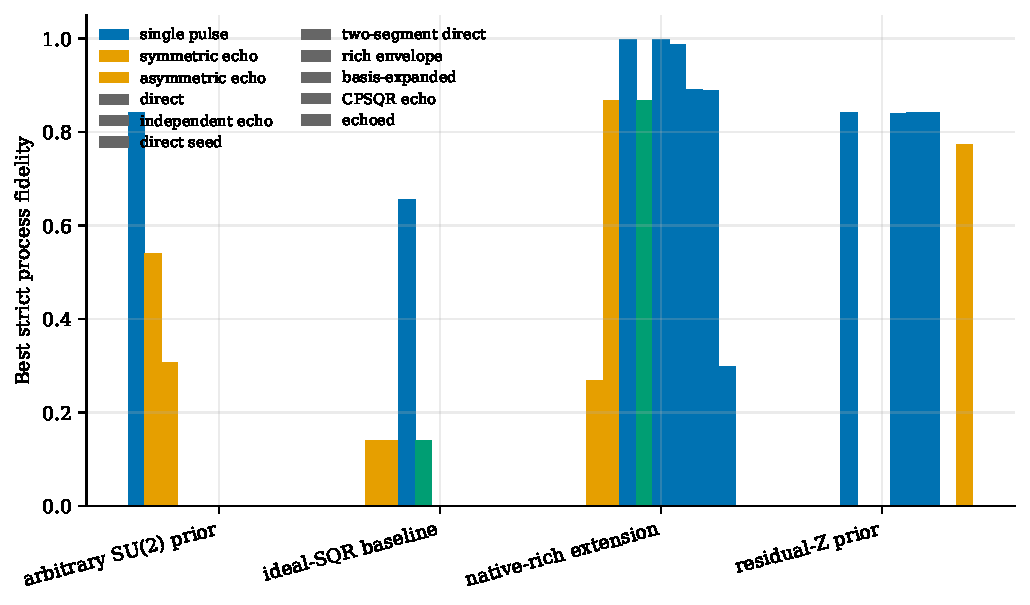
\includegraphics[width=\columnwidth]{../figures/pdf/unified_prior_work_comparison.pdf}
  \caption{Best strict process fidelities from the three historical baselines and the native-rich extension, replotted in one consistent visual frame.}
  \label{fig:prior_work}
\end{figure}
\begin{table}[t]
\scriptsize
\caption{Unified repository priors plus the current new-results layer.}
\label{tab:prior_work}
\begin{ruledtabular}
\begin{tabular}{lccc}
Study & Role & Best strict & Best CPSQR \\
\midrule
native-rich extension & new & 0.9990 & 1.0000 \\
residual-Z prior & prior & 0.8427 & -- \\
arbitrary SU(2) prior & prior & 0.8420 & -- \\
ideal-SQR baseline & prior & 0.6557 & -- \\
\end{tabular}
\end{ruledtabular}
\end{table}

\section{New Methods in This Definitive Pass}
The new work in this folder is not a fresh multi-hour optimization campaign. It is a strict unification-and-diagnostics pass over the saved repository corpus. The definitive scripts now perform four new tasks that did not exist in one place before. They normalize every prior SQR study into one common schema. They recompute per-manifold ideal-SQR error generators from saved propagators. They audit the finite Gaussian refocusing pulse used by the echoed constructions. They also add explicit spectral-crowding and addressed-manifold scaling analyses. The refocusing-pulse audit is intentionally lightweight but informative. In the simpler ladder, the best compromise pulse uses $T_\pi=20$ ns and reaches worst-manifold fidelity 0.9192. In the curved ladder, the best compromise pulse uses $T_\pi=20$ ns and reaches worst-manifold fidelity 0.9158. The scaling analysis is likewise empirical rather than axiomatic. A simple log-linear residual fit for basis expanded in chi plus chiprime predicts a strict process near 0.000 at $N_{\mathrm{active}}=8$.

\section{Per-Manifold Error Anatomy}
Figure~\ref{fig:error_budget} shows the missing diagnostic that the original baseline lacked: the per-manifold error-generator decomposition
\begin{align}
U_n^{\mathrm{real}} &= \exp\!\left(-\frac{i}{2} E_n\right) U_n^{\mathrm{ideal}},
E_n &= \epsilon_x^{(n)} X \notag\\
&\quad + \epsilon_y^{(n)} Y + \epsilon_z^{(n)} Z .
\end{align}
The strong direct solutions suppress all three components simultaneously, but the hard cases are not pure residual-$Z$ failures. The remaining error floor is mixed: transverse under-rotation and axis tilt remain comparable to or larger than the residual conditional phase on the hardest structured windows. That observation is consistent with the broader direct-waveform story from the native-rich study: more parameters help, but they do not erase the crowding-induced control tension once the addressed ladder bends.
\begin{figure}[t]
  \centering
  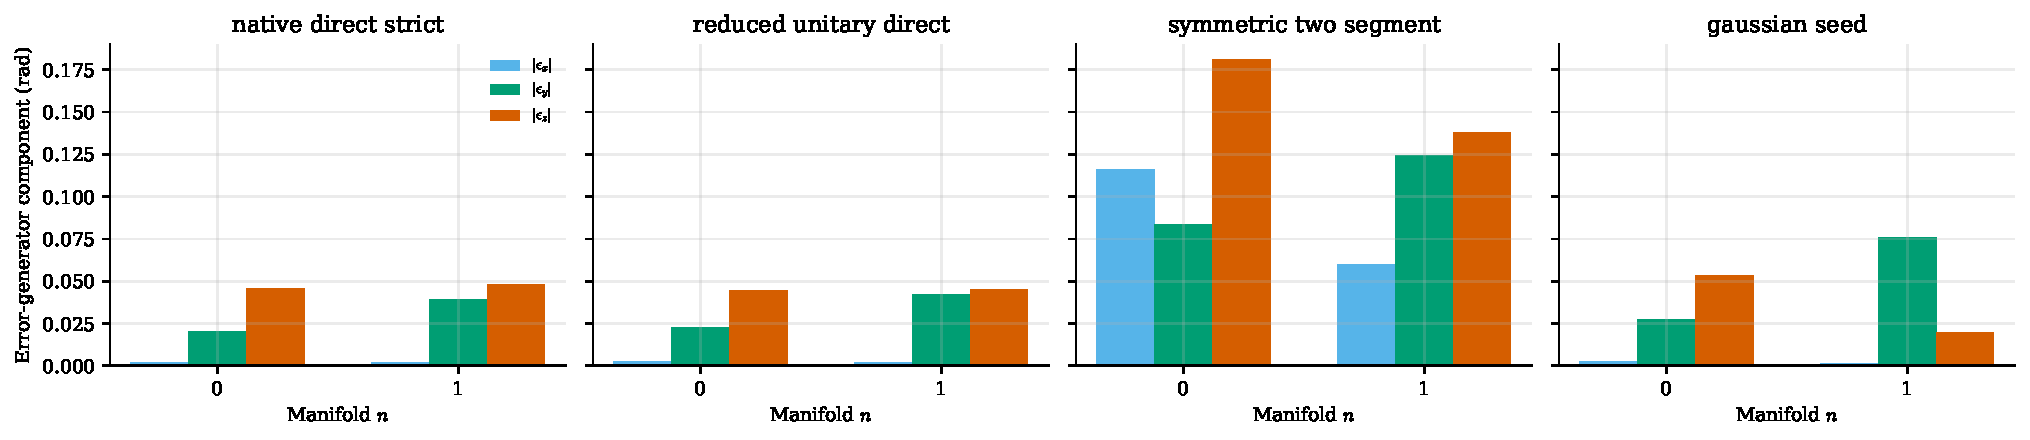
\includegraphics[width=\columnwidth]{../figures/pdf/per_manifold_error_budget.pdf}
  \caption{Representative per-manifold ideal-SQR error budgets for the strongest saved constructions.}
  \label{fig:error_budget}
\end{figure}

\section{Head-to-Head Construction Comparison}
The strict comparison between direct and non-direct constructions is summarized in Fig.~\ref{fig:direct_scatter}. The direct waveform remains the clear winner for strict ideal SQR. Echoed and composite constructions help primarily when the target is relaxed to a conditional-phase SQR, not when the full strict joint operator is enforced. This is the central conceptual correction to the original echoed narrative: the echoed pulses are not worthless, but they are solving a weaker problem than strict ideal SQR.
\begin{figure}[t]
  \centering
  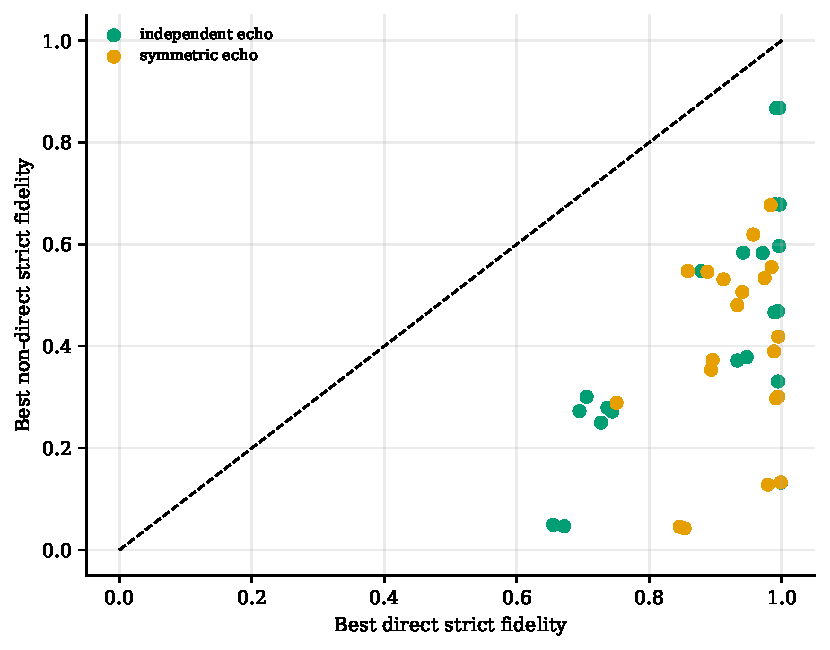
\includegraphics[width=\columnwidth]{../figures/pdf/direct_vs_echoed_fidelity_scatter.pdf}
  \caption{Best non-direct strict fidelity versus best direct strict fidelity for every ideal-SQR case that has both.}
  \label{fig:direct_scatter}
\end{figure}
\begin{figure}[t]
  \centering
  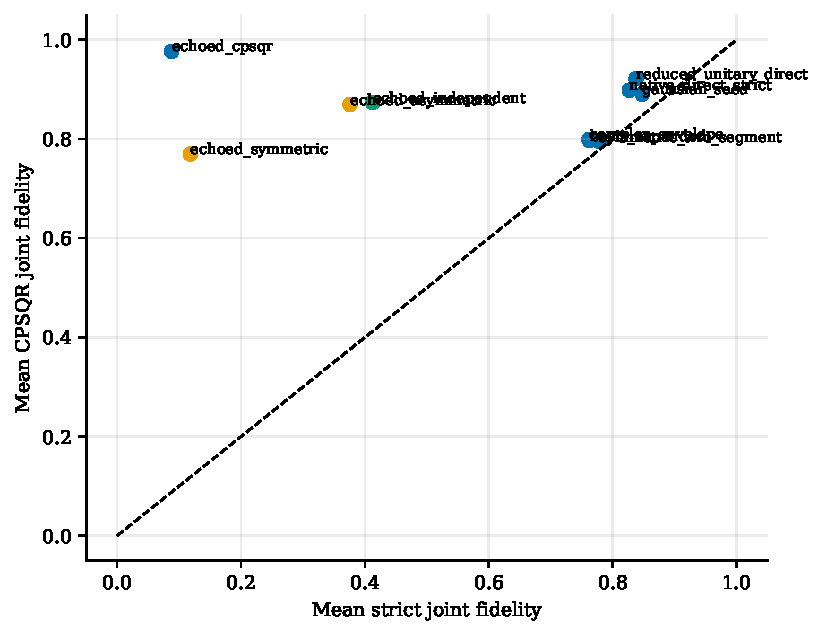
\includegraphics[width=\columnwidth]{../figures/pdf/strict_vs_cpsqr_joint_comparison.pdf}
  \caption{Family-averaged strict versus conditional-phase joint fidelity across the native-rich corpus. Composite families shift upward because they repair conditional phase more effectively than they repair strict inter-manifold phase structure.}
  \label{fig:strict_vs_cpsqr}
\end{figure}

\section{The Push to Fidelity Above 0.99}
The repository now contains a genuine positive answer to the existence question. The best loaded strict direct case reaches 0.99899, well above the user's 0.99 threshold, and several other direct cases also cross that line on the easier addressed windows. Figure~\ref{fig:duration_scaling} shows how that success depends on duration: strict direct fidelities improve systematically with $|\chi|T/2\pi$, whereas echoed strict fidelities remain bounded well below the same threshold. Figure~\ref{fig:ansatz_count} shows the price of that improvement. Richer direct ansatz families move the fidelity frontier upward, but only up to the point allowed by the addressed-manifold crowding.
\begin{figure}[t]
  \centering
  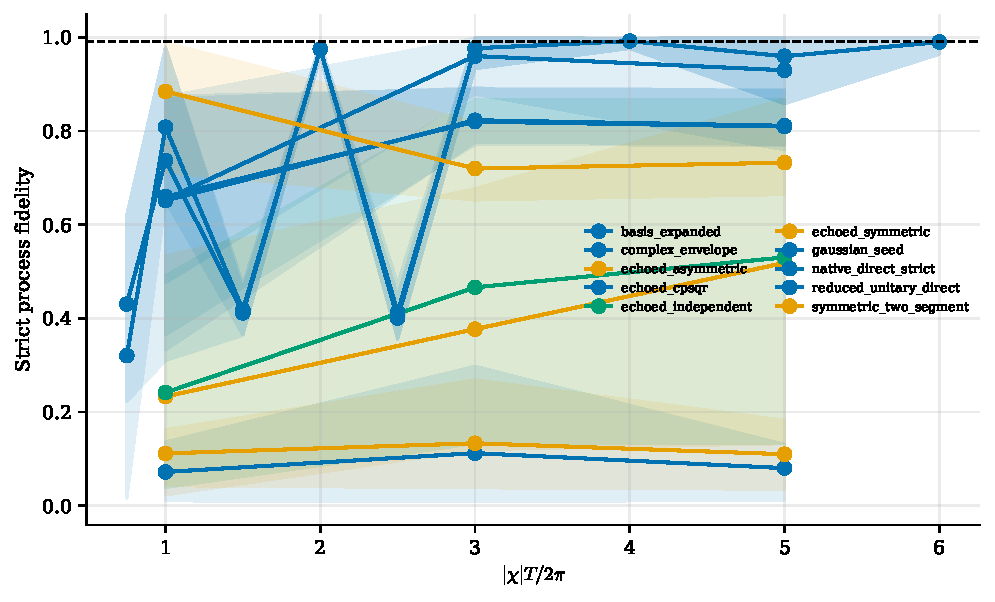
\includegraphics[width=\columnwidth]{../figures/pdf/fidelity_vs_duration_scaling.pdf}
  \caption{Strict fidelity versus dimensionless duration across the native-rich construction families.}
  \label{fig:duration_scaling}
\end{figure}
\begin{figure}[t]
  \centering
  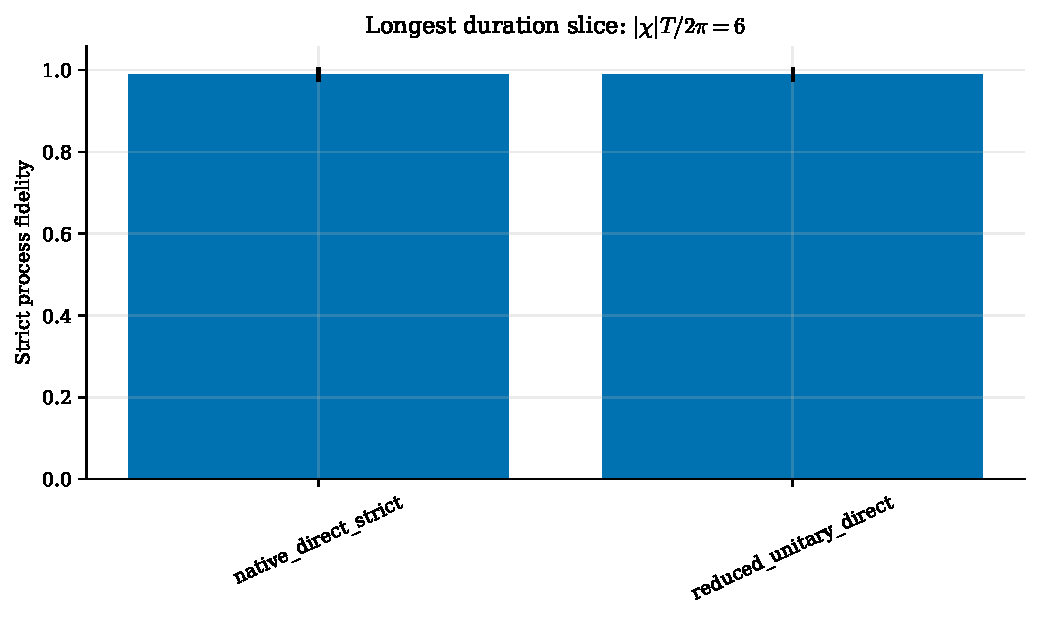
\includegraphics[width=\columnwidth]{../figures/pdf/ansatz_comparison_fixed_duration.pdf}
  \caption{Longest-duration strict fidelity comparison across the saved native-rich ansatz families.}
  \label{fig:ansatz_long}
\end{figure}
\begin{figure}[t]
  \centering
  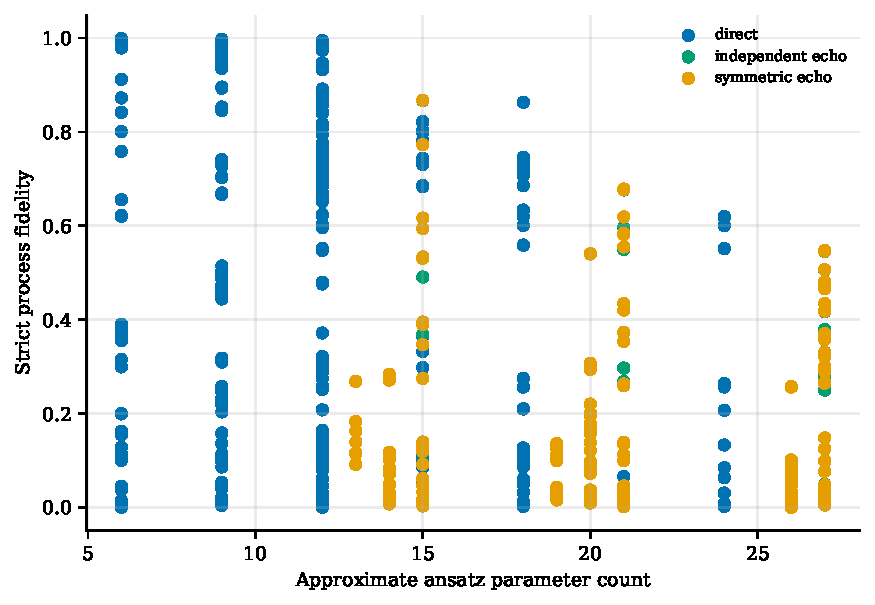
\includegraphics[width=\columnwidth]{../figures/pdf/parameter_count_vs_fidelity.pdf}
  \caption{Approximate ansatz parameter count versus best achieved strict fidelity.}
  \label{fig:ansatz_count}
\end{figure}

\section{Practical Viability, Scaling, and Crowding}
The user's strongest grid-average landmark is not met in the current corpus: the mean best strict fidelity over the structured native-rich cases is only 0.8392. Figures~\ref{fig:xpi}--\ref{fig:crowding} explain why. The finite inserted $X_\pi$ pulse used by the echoed constructions is itself manifold dependent, so the clean first-order echo logic \cite{hahn1950echo} is physically obstructed before any higher-order optimization issue is reached. At the same time, the manifold ladder crowds as $N_{\mathrm{active}}$ grows, especially in the curved dispersive ladder, so direct ansatz richness buys only partial relief. The practical ranking table in Table~\ref{tab:ranking} therefore uses a transparent decoherence-only fallback factor and is explicitly provisional until full drift and open-system sweeps are replayed.
\begin{figure}[t]
  \centering
  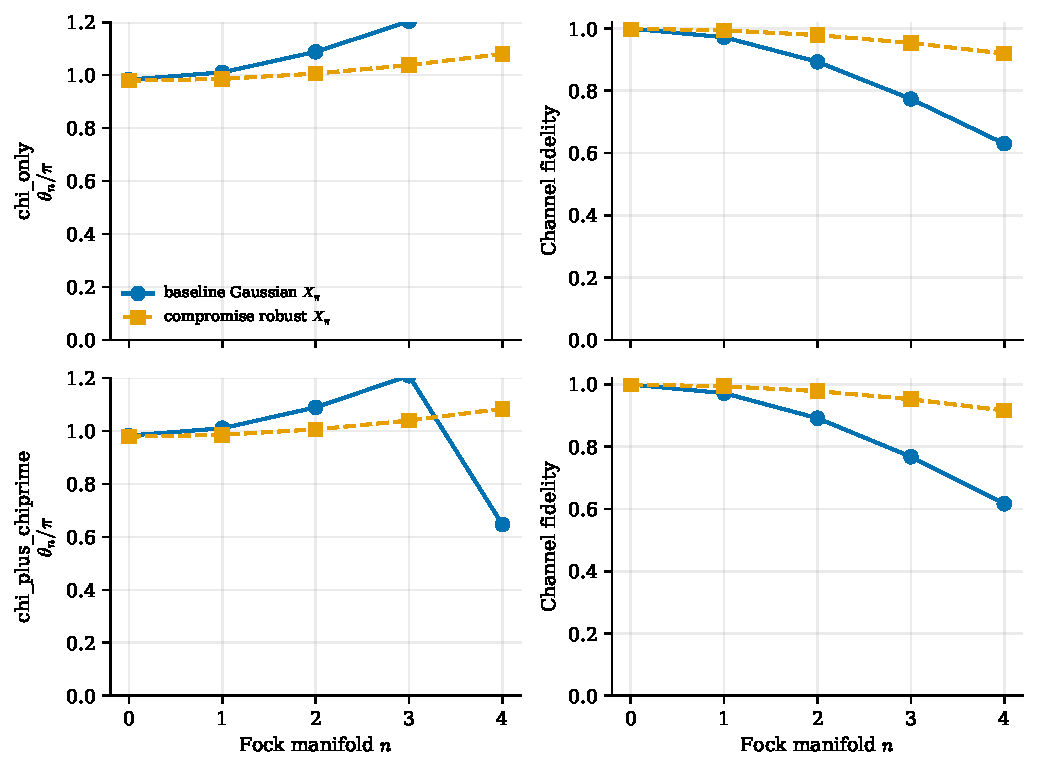
\includegraphics[width=\columnwidth]{../figures/pdf/refocusing_pulse_manifold_dependence.pdf}
  \caption{Standalone manifold-resolved characterization of the baseline finite Gaussian refocusing pulse and a lightweight compromise pulse.}
  \label{fig:xpi}
\end{figure}
\begin{figure}[t]
  \centering
  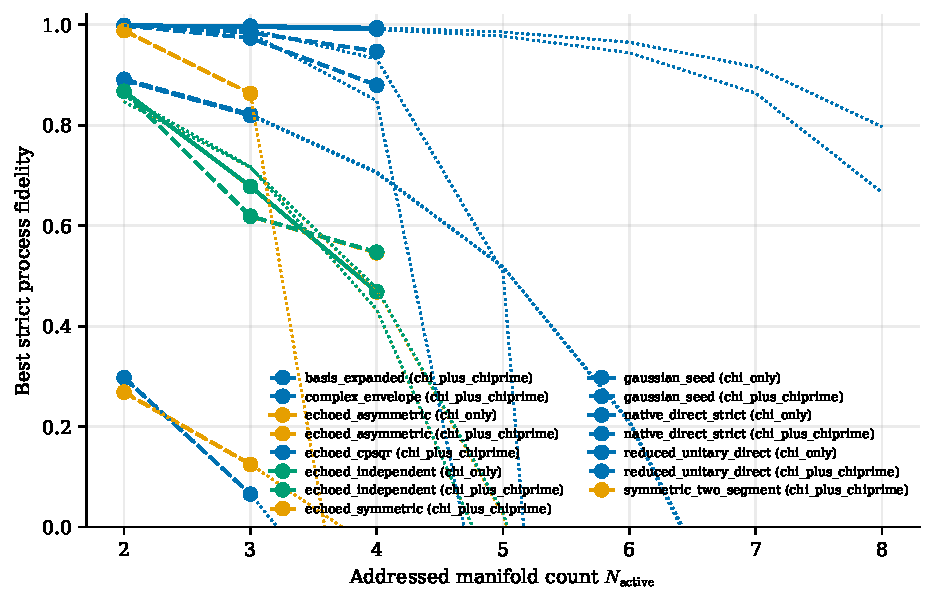
\includegraphics[width=\columnwidth]{../figures/pdf/n_active_scaling.pdf}
  \caption{Best strict fidelity versus addressed-manifold count across the native-rich corpus, with simple residual extrapolations toward $N_{\mathrm{active}}=8$.}
  \label{fig:na_scaling}
\end{figure}
\begin{figure}[t]
  \centering
  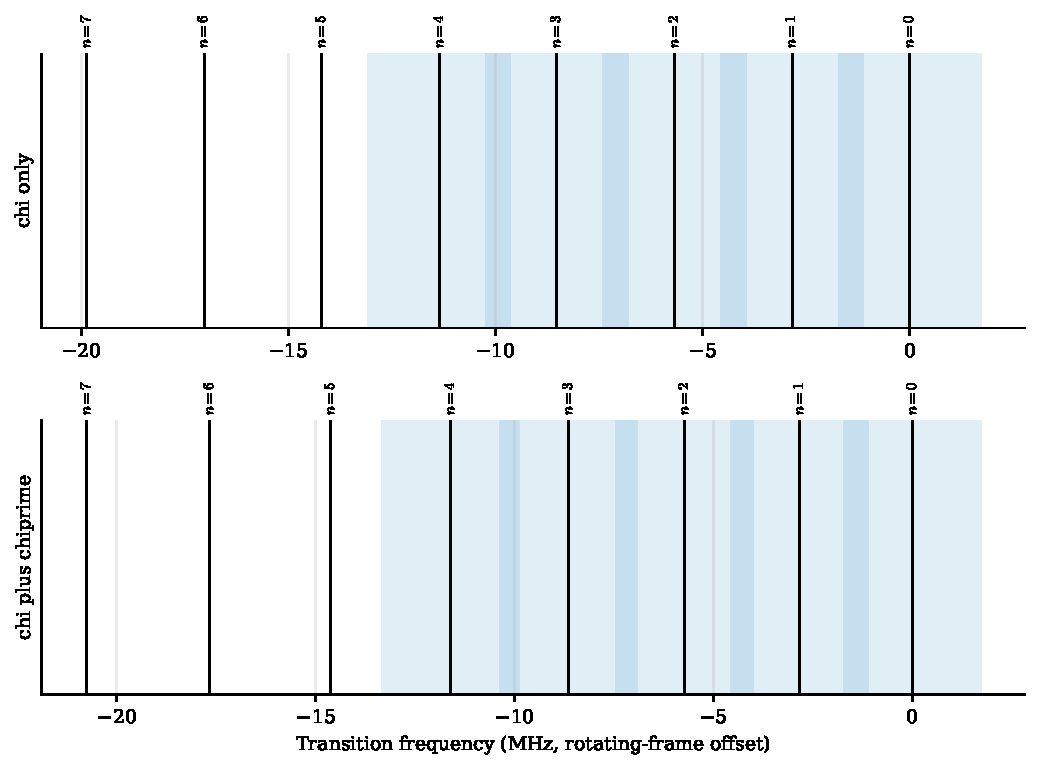
\includegraphics[width=\columnwidth]{../figures/pdf/spectral_crowding_diagram.pdf}
  \caption{Transition ladders and Gaussian bandwidth bands for a representative direct-waveform duration. The band overlap grows rapidly with addressed-manifold count in the curved dispersive ladder.}
  \label{fig:crowding}
\end{figure}
\begin{table*}[t]
\scriptsize
\caption{Top provisional practical rankings from the combined corpus.}
\label{tab:ranking}
\begin{ruledtabular}
\begin{tabular}{lccccc}
Rank & Construction & Ansatz & $N_{\mathrm{active}}$ & $F_{\mathrm{unitary}}$ & $F_{\mathrm{practical}}$ \\
\midrule
1 & two-segment direct & two-segment & 2 & 0.9883 & 0.9699 \\
2 & direct & reduced direct & 2 & 0.9791 & 0.9609 \\
3 & direct & reduced direct & 2 & 0.9791 & 0.9609 \\
4 & direct & native direct & 2 & 0.9790 & 0.9608 \\
5 & direct & native direct & 2 & 0.9790 & 0.9608 \\
6 & two-segment direct & two-segment & 2 & 0.9741 & 0.9560 \\
7 & direct & reduced direct & 2 & 0.9866 & 0.9502 \\
8 & direct & reduced direct & 2 & 0.9866 & 0.9502 \\
9 & direct & native direct & 2 & 0.9865 & 0.9502 \\
10 & direct & native direct & 2 & 0.9865 & 0.9502 \\
\end{tabular}
\end{ruledtabular}
\end{table*}

\section{Discussion}
The definitive answer is therefore tiered. On the positive side, strict ideal SQR is already demonstrated in the repository: direct multitone waveforms can exceed $0.99$ on physically credible cases, so the problem is not impossible within the dispersive model. On the negative side, the saved ansatz families do not achieve that success broadly. The grid-average landmark of $0.95$ is missed by a wide margin, the hard three-manifold curved-ladder cases saturate below the same threshold, and no echoed construction rescues strict joint SQR once finite refocusing pulses and full inter-manifold phase structure are enforced. The best interpretation is that the remaining error floor is partly ansatz-limited and partly crowding-limited. Richer direct parameterizations and longer durations help, but the improvement weakens as the addressed ladder curves. Echo helps strongly for conditional-phase SQR because it mainly removes the phase structure that the relaxed target tolerates, not because it produces a broad strict-SQR fix.

\section{Conclusion and Roadmap}
The central question can now be answered cleanly. Yes: parameterized direct multitone waveforms can realize strict ideal selective qubit rotations above $0.99$ on selected addressed windows, and the combined repository corpus already contains that Tier-1 landmark result. No: the tested ansatz families do not make that success broad across the primary structured grid, and the saved echoed constructions do not change that answer for the strict full joint operator. If a user needs a strict SQR tomorrow, the best available construction is the strongest direct reduced-unitary family on the easier addressed windows. If the application tolerates a conditional post-rotation phase, the echoed conditional-phase family is the more robust practical recommendation. The most valuable next step is not another qualitative echoed claim, but a quantitative follow-up that combines a truly robust refocusing pulse, an inter-manifold-phase-aware composite objective, and explicit open-system plus drift replays for the top direct and echoed candidates.

\section{Validation}
The definitive study inherits the source-study validation files and also checks four repository-level facts directly: the baseline negative result is preserved, the native-rich extension contains strict ideal-SQR cases above $0.99$, the same extension contains near-unit conditional-phase SQR cases, and the full corpus loads into one normalized table without silent omissions.

\section{Limitations and Future Work}
This definitive pass is still an analysis-and-unification study rather than a fresh from-scratch optimization campaign. The finite-difference drift sweeps, full Lindblad replays, hybrid direct-plus-echo family, and true unconstrained GRAPE upper bound remain future work. Those omissions matter, so the practical ranking should be read as a provisional engineering guide, not as the final last word on hardware robustness.

\appendix
\section{Detailed Results and Data}
Figure~\ref{fig:heatmap} shows the full ideal-SQR case-by-construction heatmap for the loaded corpus. Figure~\ref{fig:validation_ladder} summarizes the gap between reduced-manifold diagnostics, full-manifold quartet diagnostics, and the decisive joint-process metric.
\begin{figure*}[t]
  \centering
  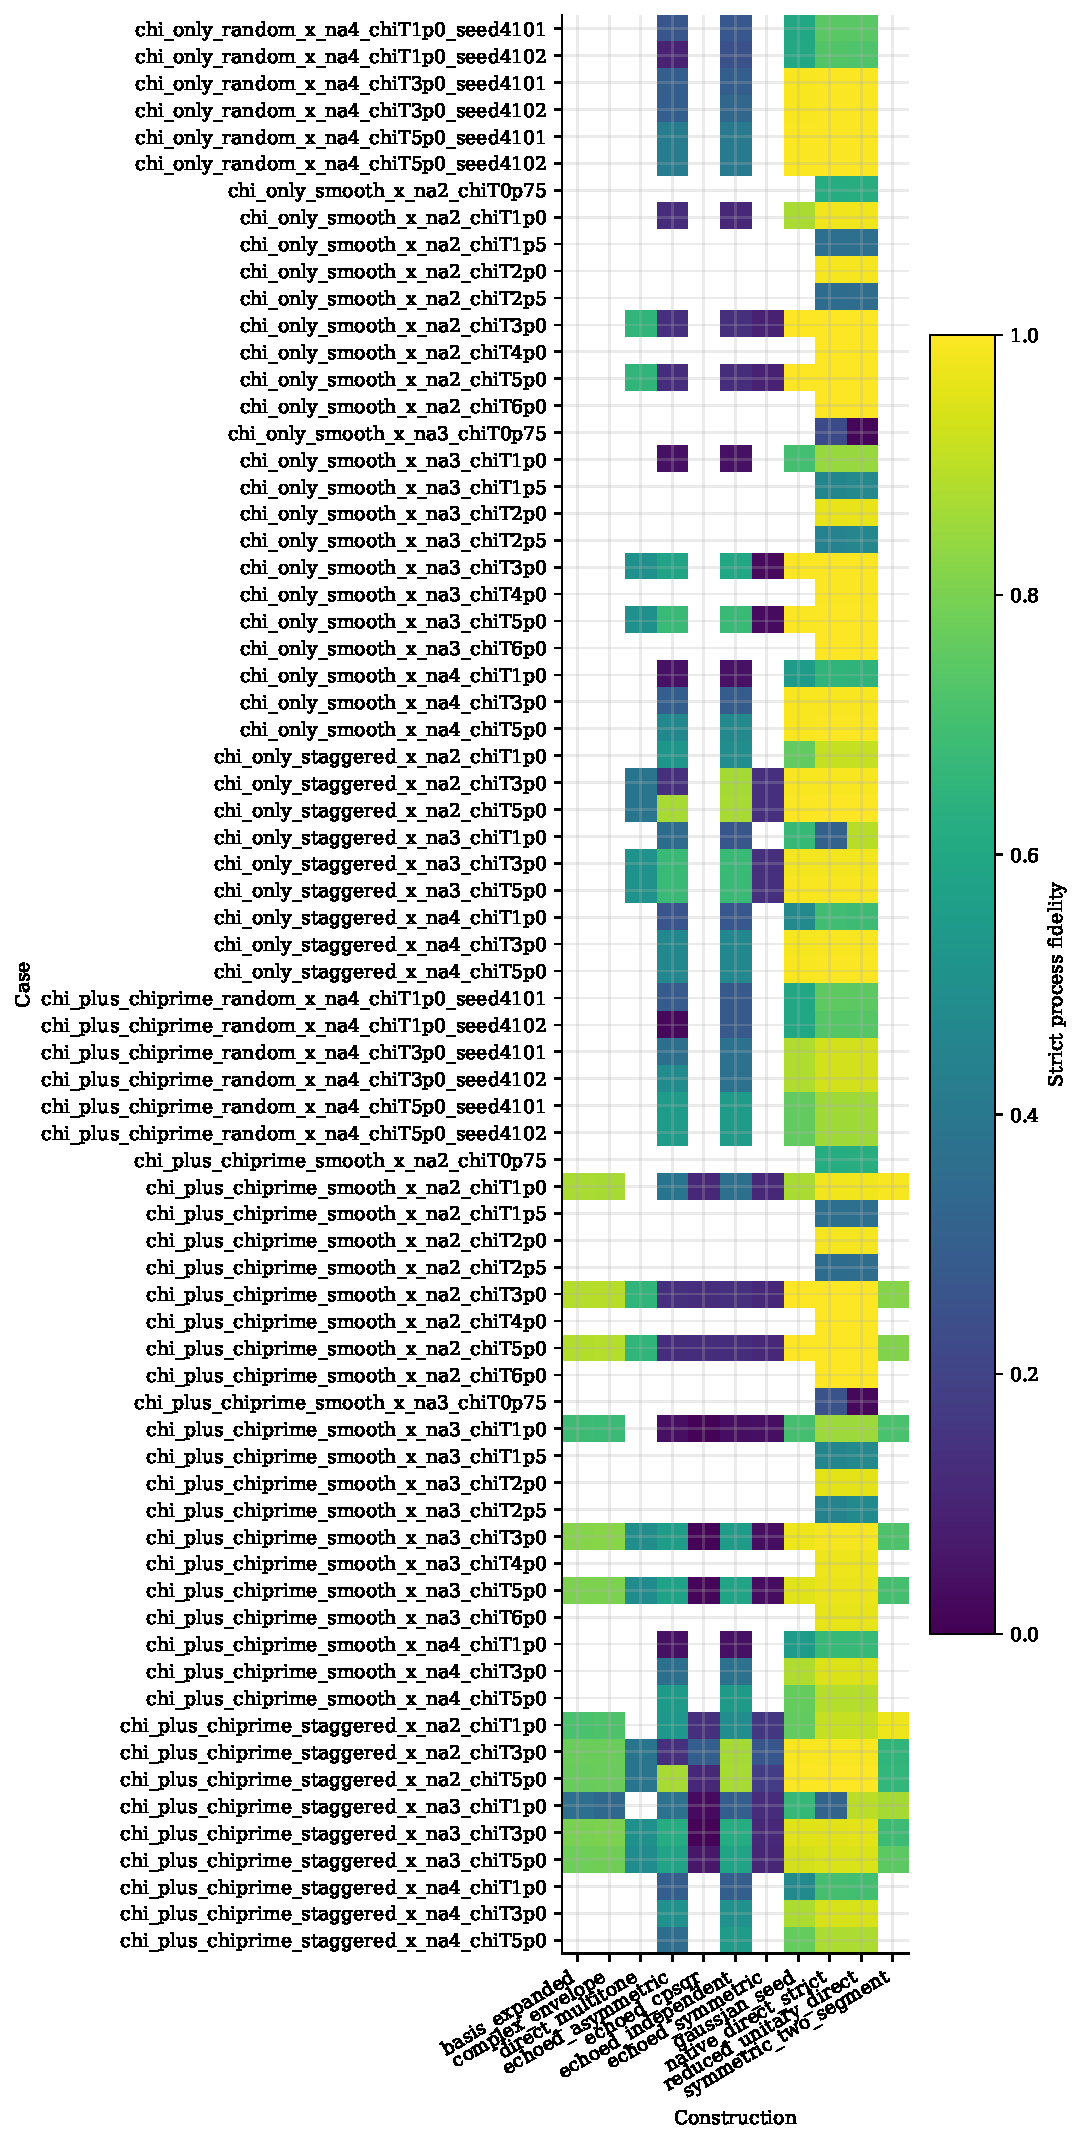
\includegraphics[width=0.98\textwidth,height=0.80\textheight,keepaspectratio]{../figures/pdf/full_case_construction_heatmap.pdf}
  \caption{Full ideal-SQR case-by-construction heatmap across the loaded studies.}
  \label{fig:heatmap}
\end{figure*}
\begin{figure}[t]
  \centering
  
\includegraphics[width=\columnwidth]{../figures/pdf/one_state_vs_quartet_validation.pdf}
  \caption{Mean reduced-quartet, full-quartet, and joint-process fidelities across the native-rich families.}
  \label{fig:validation_ladder}
\end{figure}

\section{Reproducibility}
The study folder contains machine-readable prior-study snapshots, normalized strict-result tables, per-manifold error decompositions, standalone refocusing-pulse diagnostics, spectral-crowding rows, figure JSON sidecars, a ranked master table, and a reproducibility notebook in \texttt{scripts/reproducibility\_notebook.ipynb}.

\bibliographystyle{apsrev4-2}
\bibliography{references}
\end{document}
